\newpage
\chapter{State of the Art Review}
\label{sec:stateoftheart}

In this chapter, we present a review of state-of-the-arts regarding synthetic data generation for deep neural networks to be applied for learning to count tasks. We introduce a summary of cutting-edge research studies from two aspects. First we succinctly review the background of generating synthetic data for different problems, and then a short history of feature detection algorithms will be alluded.

\section{Synthetic Data Generation} 

The main purpose of generating synthetic datasets has been to protect the privacy and confidentiality of the actual data \cite{yao2015synthetic,phua2010comprehensive}, since it does not hold any personal information and cannot be traced back by any individual. In addition, synthetic data are used to meet specific needs or certain conditions that may not be found in the original, real data. This can be useful when designing any type of system because the synthetic data are used as a simulation or as a theoretical value, situation, etc. For example, in \cite{hofmeyr1998intrusion}, the authors introduce a method for detecting intrusions where the experiment is done using synthetic data. This data is a representation of the authentic data and may include intrusion instances that are not found in the authentic data. The synthetic data allows the software to recognize these situations and react accordingly.

Furthermore, synthetic data have been applied by recent learning algorithms as a viable alternative to complement the real data where the real data is not publicly available, or quite difficult to collect \cite{hu2016frankenstein}. These datasets are generated at a high realistic state and preserve high levels of accuracy compared to the original data. For instance, in \cite{gaur2015generation}, the authors improve the performance by creating additional synthetic training data due to the lack of real dataset. Moreover, \citealt*{jaderberg2014synthetic} introduces a framework for natural scene text recognition solely by training deep convolutional neural network with synthetically generated and labeled data.

\noindent The use of synthetic data has a longstanding history in computer vision and more specifically for object detection problems. For example, \cite{shotton2013real} used synthetic dataset to propose a method for human pose prediction while In \cite{rematas2014image}, the author proposed a technique to improve novel-view synthesis for images using the structural information\footnote{Structural information theory (SIT) is a theory about human perception and in particular about visual perceptual organization, which is the neuro-cognitive process that enables us to perceive scenes as structured wholes consisting of objects arranged in space.} from 3D models. 
 
After the success of deep learning algorithms in solving various problems in computer vision by obtaining cutting-edge results, generate and use of synthetic data has been considered for training different learning algorithms as a viable alternative to complement the real data \cite{gaur2015generation,jaderberg2014synthetic}. In particular, convolutional neural networks have been used to learn from synthetically created datasets \cite{rematas2014image,gaur2015generation,jaderberg2014synthetic}. As one of the most recent approaches, \citeauthor*{segui2015learning} in \cite{segui2015learning} proposed synthetic data generation to counter lack of data issue for learning to count the number of objects in images using deep convolutional neural networks. In their work, they took advantage of existent unlabeled and labeled datasets to generate realistic synthetic images representative of the actual images. The authors introduce two counting problems, counting number of even-digits in images, and counting the amount of pedestrians in a walkway. They do their experiment solely by training deep convolutional neural networks on synthetic datasets.  
% start with an intro about synthetic datasets
% relate it to images and the way they generate it 
% mention the works in dl and recent papers

\section{Feature Detection Algorithms} 

\noindent Counting the number of an object of interest in an image can be approached from two different perspectives, either training an object detector, or training an object counter \cite{segui2015learning}. In the field of object detection, numerous works have been previously proposed \cite{paragios2001mrf, cho1999neural, regazzoni1996distributed, davies1995crowd, kong2005counting, marana1998efficacy, viola2004robust}. Most of these research works follow a taxonomy which consists of three paradigms underneath to count the objects:
\begin{enumerate}
	\item Object detection, which are based on boosting appearance and motion features \cite{viola2005detecting, viola2004robust}, Bayesian model-based segmentation \cite{zhao2003bayesian}, integrated top-down and bottom-up processing \cite{leibe2005pedestrian, oliva2003top,chan2008privacy}.
	\item Visual feature trajectory clustering. This paradigm counts objects by identifying and tracking visuals over a  time period. Feature trajectories with coherent motion are then clustered and the number of clusters is the estimate of the number of moving people \cite{rabaud2006counting, brostow2006unsupervised,chan2008privacy}. 
	\item feature-based regression. These methods usually work by first, subtracting the background, second, measuring various features of the foreground pixels such as total area \cite{paragios2001mrf, davies1995crowd}, edge count \cite{cho1999neural, regazzoni1996distributed}, or texture  \cite{marana1998efficacy}; and finally estimating the crowd density or crowd count by a regression function, e.g. linear \cite{paragios2001mrf, davies1995crowd}, piece-wise linear \cite{regazzoni1996distributed}, or neural networks \cite{cho1999neural, regazzoni1996distributed}. 

	\indent In recent years, feature-based regression has also been applied to outdoor scenes. For example, \citealt{kong2005counting} applies neural networks to the histograms of foreground segment areas and edge orientations. \citealt{dong2007fast} estimates the number of people in each foreground segment by matching its shape to a database containing the silhouettes of possible people configurations, but is only applicable when the number of people in each segment is small (empirically, less than 6)\cite{chan2008privacy}.  
\end{enumerate} 
By reason of the fact that almost all the above algorithms detect the whole objects in an image (e.g. whole pedestrians), these methods have moderate performance in very noisy or crowded images with significant occlusion, \citealt*{wu2005detection, lin2001estimation}, introduced methods to address this issue. \citealt*{wu2005detection} proposed \textit{edgelet features} (an edgelet is a short segment of line or curve) as new type of silhouette oriented features to deal with the problem of detecting individuals in crowded still images. %Respectively in \cite{lin2001estimation}, \citeauthor*{lin2001estimation} used \textit{Accumulated Mosaic Image Difference(AMID)} method to extract crowd areas having irregular motion. 

\indent As a similar line of work in the course of object counting and more specifically crowd counting, in \cite{rabaud2006counting, brostow2006unsupervised, leibe2007coupled}, different object tracking approaches were taken to detect and count moving objects in the scene. However, the deployment of these vision surveillance technologies are invariably met with skepticism by society at large, given the perception that they could be used to infringe on the individuals' privacy rights. While a number of methods that do not require explicit detection or tracking have been previously proposed \cite{paragios2001mrf, cho1999neural, regazzoni1996distributed, davies1995crowd, kong2005counting, marana1998efficacy, dong2007fast}, they have not fully established the viability of the privacy-preserving approach\cite{chan2008privacy}. The tension of privacy-preserving is common in all areas of data-mining \cite{vaidya2006privacy, verykios2004state}. 

In order to tackle privacy preserving issue, \citealt*{chan2008privacy} presented a novel approach with no explicit object segmentation or tracking to estimate the number of people moving in each direction(towards and away from camera) in a privacy-preserving manner. An outline of the crowd counting system appears in figure~\ref{fig:ucsd}:
\begin{figure}[H]
	\centering
	{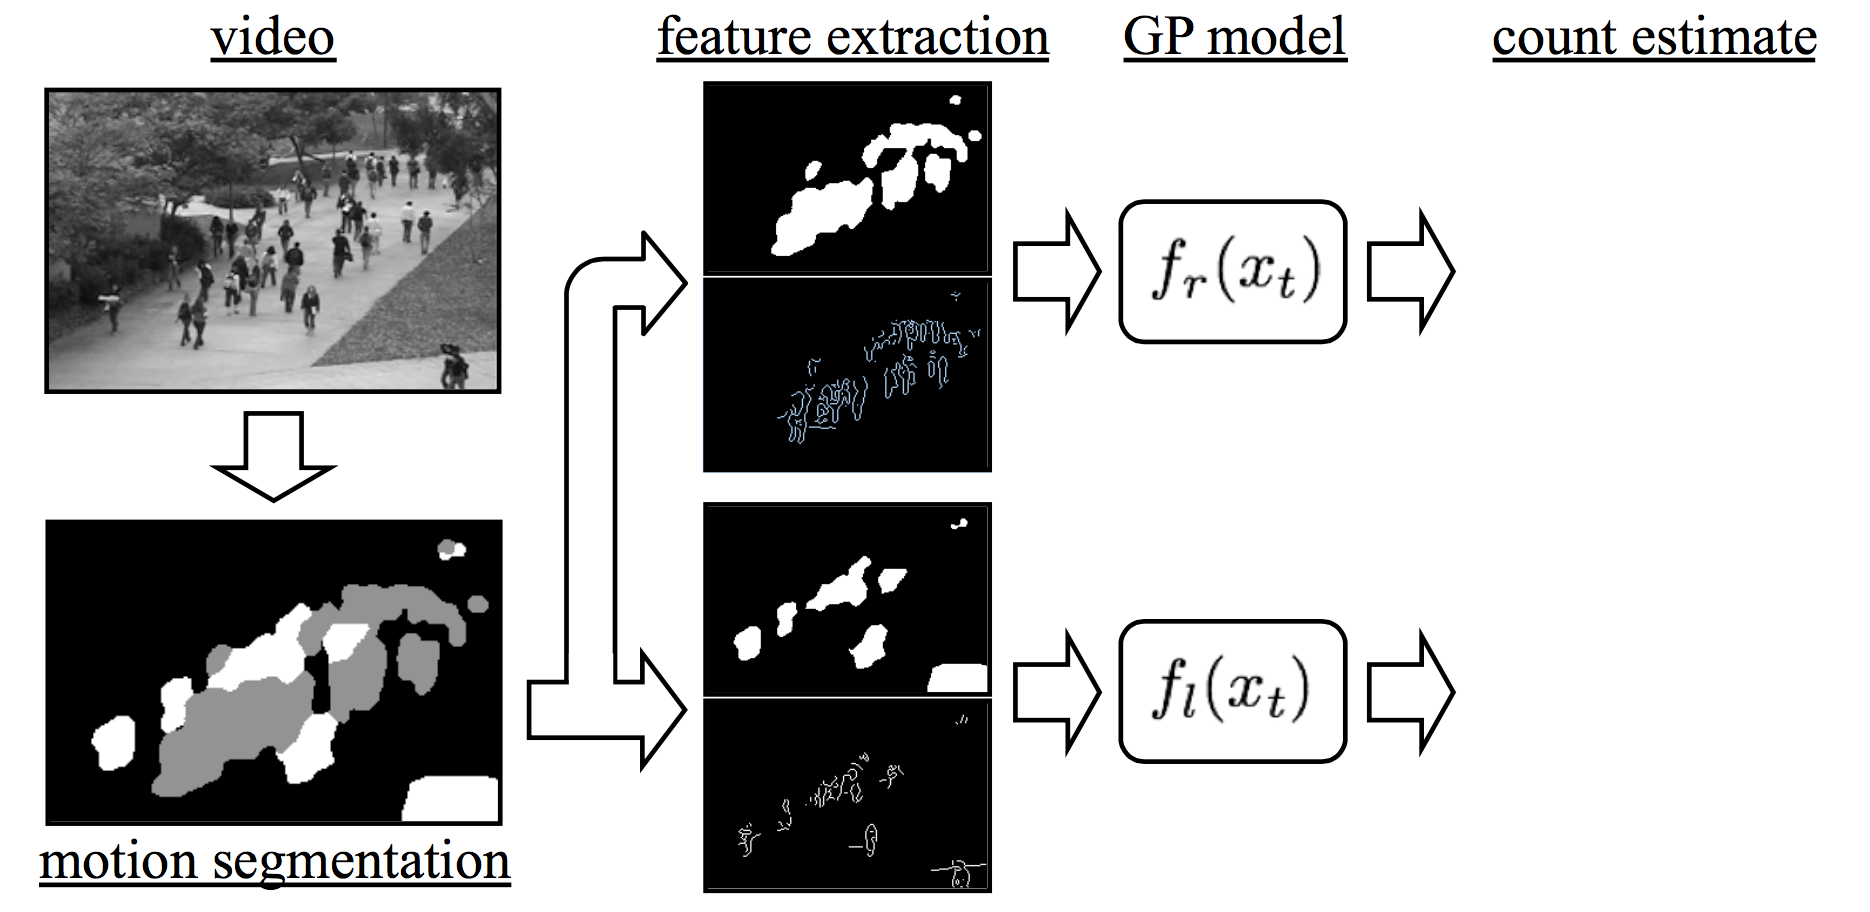
\includegraphics[width=0.8\textwidth]{images/ucsdOutline}}
	\caption{Crowd counting system: the scene is segmented into crowds with different motions. Normalized features that account for perspective are extracted from each segment, and the crowd count for each segment is estimated with a Gaussian process\cite{chan2008privacy}.}
	\label{fig:ucsd}
\end{figure}

\citeauthor*{chan2008privacy} used a mixture of \textit{dynamic textures}\footnote{Dynamic textures are sequences of images of moving scenes that exhibit temporal regularity, intended in a statistical sense, like sea-waves, smoke, foliage, whirlwind but also talking faces, traffic scenes etc.} \cite{doretto2003dynamic, chan2008modeling} to divide the video frames into regions containing moving pedestrians in different directions. When adopting mixture of dynamic textures, the video is represented as collection of spatio-temporal patches which are modeled as independent samples from mixture of dynamic models \cite{doretto2003dynamic}. The mixture model is learned through Expectation-Maximization(EM) algorithm \cite{chan2008modeling}. Video locations are then scanned sequentially, a patch is extracted at each location, and assigned to the mixture component of largest posterior probability. The location is declared to belong to the segmentation region associated with that component  \cite{chan2008privacy}. The resulting segmentations of their work are illustrated in figure~\ref{fig:segUcsd}:
\begin{figure}[H]
	\centering
	{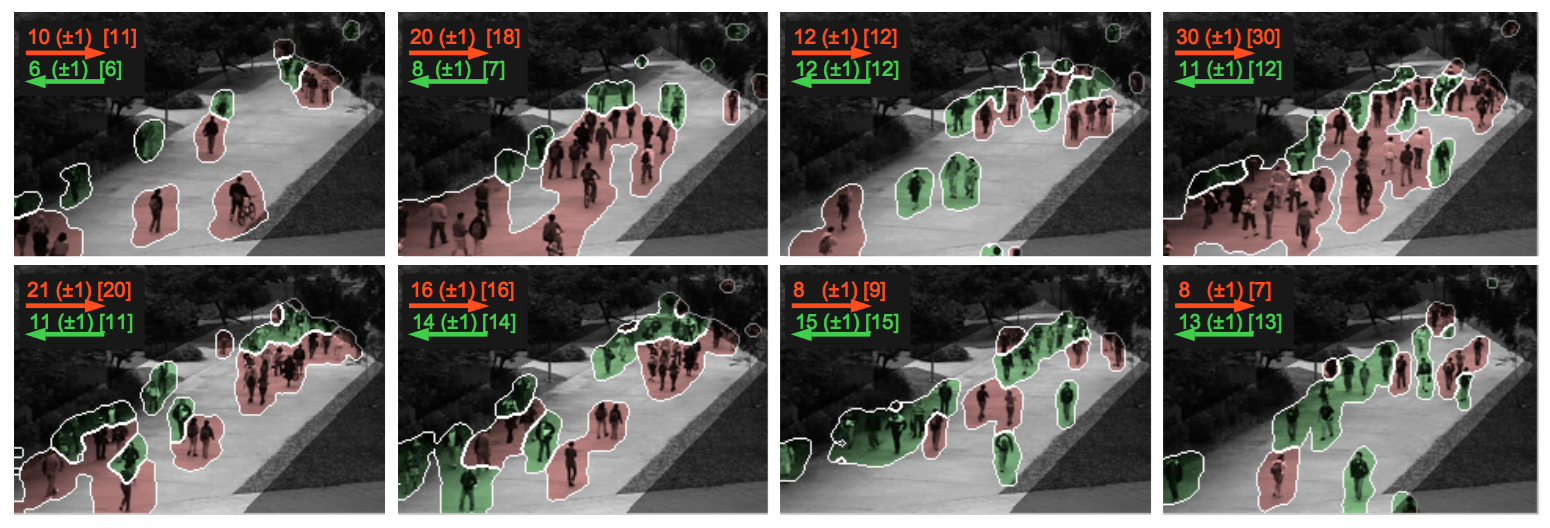
\includegraphics[width=0.9\textwidth]{images/segUcsd}}
	\caption{Crowd counting results: The red and green segments are the “away” and “towards” crowds. The estimated crowd count for each segment is in the top-left, with the (rounded standard-deviation of the GP) and the ground-truth. The Region Of Interest (the area in the walkway in which the pedestrians are counted and labeled) is also highlighted \cite{chan2008privacy}.}
	\label{fig:segUcsd}
\end{figure}

After segmenting the moving pedestrians, extracting features from the video segments is done at three phases:
\begin{itemize}
	\item Segment features to capture segment shape and size. Features such as area, perimeter, perimeter edge orientation and perimeter-area ratio. 
	\item Internal edge features contained in a crowd segment are a strong about the number of pedestrians in the segment \cite{davies1995crowd, kong2005counting}. For instance, total edge pixels and edge orientation. 
	\item Texture features which are based on gray-level co-occurrence matrix(GLCM) (see  \cite{haralick1973textural} for more details) were applied for image patches classification into 5 classes of crowd density in \cite{marana1998efficacy}. Due to the task similarity, \citeauthor*{chan2008privacy} adopted a similar set of measurements for counting the number of crowd in each segment, and computed texture properties like homogeneity, energy and entropy. 
\end{itemize} 

Having features from the segments extracted, a Gaussian Process(GP) \cite{williams2006gaussian} was used to regress feature vectors to the number of people per segment. The GP defines a distribution over functions, which is “pinned down” at the training points \cite{chan2008privacy}. Since the classes of function that GP can model is directly dependent on the chosen kernel function, they combined the linear and the squared-exponential(RBF)(see \cite{chang2010training, vert2004primer, shashua2009introduction} for more details) kernels, \textit{i.e.}
\begin{equation}
\centering k(x_p, x_q) = \alpha_1(x_p^{T}x_q+1) + \alpha_2e^{\frac{-\|x_p-x_q\|^2}{\alpha_3}} + \alpha_4\delta(p,q)     
\end{equation}
The linear component of the kernel captures the dominant trend of many features which is linear(\textit{e.g.} segment area), while the RBF component models local non-linearities that arise from a variety of factors, including occlusion, segmentation errors and pedestrian configuration (\textit{e.g.} spacing within a segment) \cite{chan2008privacy}. 
  
For this experiment, they collected an hour of video from a stationary digital camera. The first 2000 frames of the videos were annotated as ground-truth. Moreover, a region-of-interest(ROI) was selected on the walkway(see figure~\ref{fig:segUcsd}), and the traveling directions (away from or towards the camera) and visible center of each pedestrian was annotated. Then the video was split into a training set, for learning the GP, and a test set for validation. The training set contains 800 frames, between frame 600 and 1399, with the remaining 1200 frames held out for testing. This dataset is available to the vision community \cite{chan2008privacy}.

The obtained results for crowd counting in  \cite{chan2008privacy} are expressed as both mean-squared-error(MSE) and mean-absolute-error(MAE) between the estimate and ground-truth. This reasonable results given the small dataset and also its' privacy-preserving manner notwithstanding, this work, like the aforementioned methods, requires not only exhaustive data annotations and large training set, but also hand-crafting highly specialized image features that are dependent on the object class. 

%However, if the problem is tackled from the perspective of object counters and not object detectors, we only need to provide the number of object instances for each image sample and the result is typically a regressor\cite{lempitsky2010learning}.  

In order to save annotation efforts, different techniques were used to count objects. Multiple Instance Learning(MIL) \cite{foulds2010review} is a variation of supervised learning in which instances come in bags. These bags contain multiple samples. A bag is labeled positive if there is at least one example with the concept of interest, or labeled negative otherwise. The positive bag can be regarded as a set of attracting instances and the negative one as a set of repulsive instances. In large-scale Computer Vision, this approach is frequently found under the name of \textit{weakly supervised learning} \cite{weber2000unsupervised, fergus2003object}. There are different definitions for the term "weakly" in the literature. For instance, in \cite{dekel2009good}, it is a surrogate for the concept of noisy labels such as labels provided by different supervisors with distinct quality. However, in \cite{raykar2009supervised}, it is described for indicating imperfect annotation or even in \cite{wang2013weakly} for specifying only the presence of an object in an image. 

\indent Early works used weakly supervised learning in an instantiation of the MIL framework for for inferring difficult to describe classes such as in \cite{todorovic2006extracting} where photometric, geometric, and topological features are recognized. More recently, several works, such as \cite{nguyen2009weakly}, explore the capacity of this technique for simultaneous localization and recognition. Another work using MIL framework was count-based multiple instance learning \cite{foulds2010review}. In count-based MIL the positive bag is composed of instances where the concept appears within the range of an interval. For example, the positive bag may contain images with 5 to 10 appearances of pedestrians. A major drawback of MIL framework is that even in count-based MIL the problem is casted as a binary task and they would not be applicable in projects where the exact number of objects in the image important. 

Furthermore, another approach to reduce the annotation tasks is done in \cite{flaccavento2011learning}, where the labeling process is decreased to dotting(pointing) and the counting process is addressed as image density estimation problem.  

Recently, with the success of CNNs in different vision tasks, object detection systems based on deep CNN have made groundbreaking advances on several object detection problems \cite{zhang2015improving, erhan2014scalable, girshick2014rich, he2015spatial, erhan2014scalable} which suggests the use of this technique to learn to count objects. Several advantages can be foreseen from this application, being the most important that of learning image features from samples instead of hand-crafting highly specialized image features that are dependent on the object class \cite{segui2015learning}. Moreover, CNN have shown their capacity of knowledge transfer for a number of tasks or the ability of simultaneously performing different tasks even when trained for only one \cite{zhou2014learning}. 

Following this line of work,  \citefullauthor{segui2015learning} in \cite{segui2015learning} proposed a novel approach for counting objects' representations using deep object features. In their work, objects' features are learned by a deep counting convolutional neural network and are used to understand the underlying representation. Their proposal lies in the middle of weakly supervised learning and fully supervised learning \cite{mohri2012foundations}. It is similar to weakly supervised learning because the location of the concept of interest is not given. Whereas, unlike fully supervised learning in which the object boundary or bounding box is given to the learning process, in their proposed architecture, only the multiplicity of the object is provided \cite{segui2015learning}.

To this end, they defined a counting problem for even digits using \textit{MNIST} data and demonstrated that the internal representation of the network is able to classify digits in spite of the fact that during training, no direct supervision was provided. Moreover, they present preliminary results about a deep network that is able to count the number of pedestrians in a scene \cite{segui2015learning}. Figure~\ref{fig:santimnist} illustrates their proposal at a glance in the case of representing hand-written digits:
\begin{figure}[H]
	\centering
	{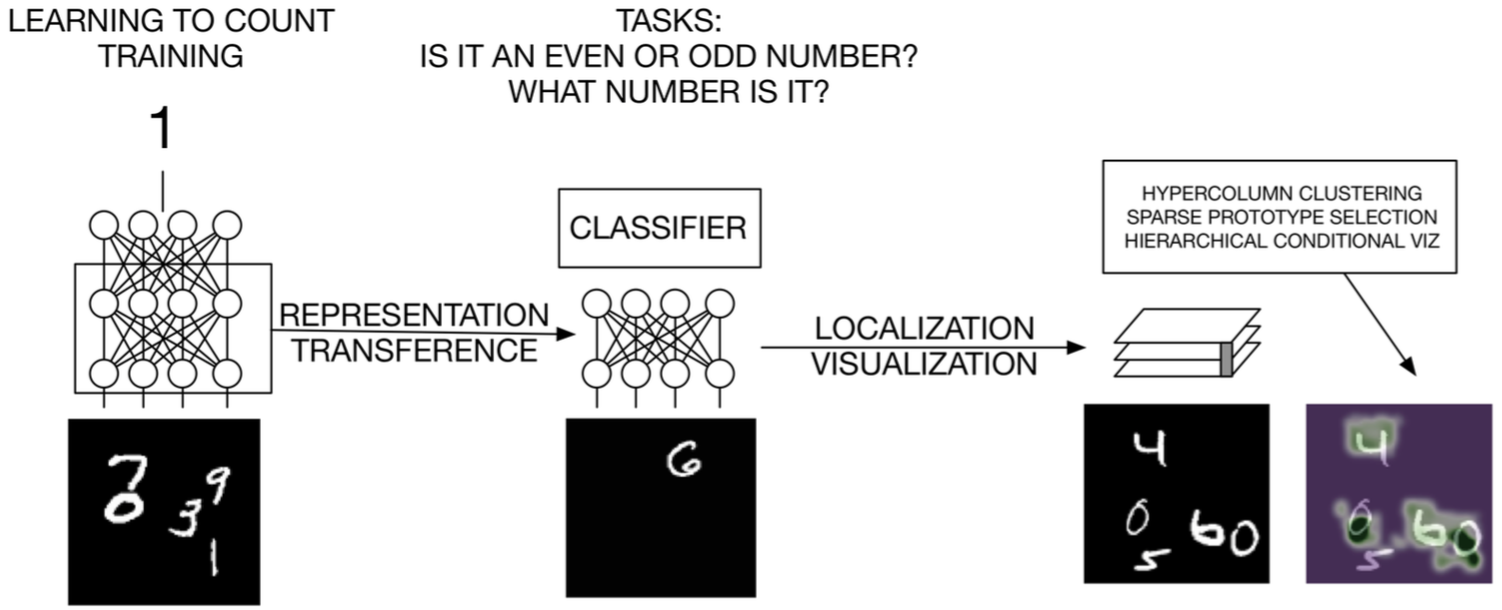
\includegraphics[width=0.9\textwidth]{images/santimnist}}
	\caption{Learning to count hand-written digits problem in which the features of a CNN that has been trained to count digits can be readily used for more specific classification problems and even to localize digits in an image\cite{segui2015learning}.}
	\label{fig:santimnist}
\end{figure}

In \cite{segui2015learning}, the main hypothesis is that the number of occurrence of objects in an image provide strong presentational information due to their possible discriminate appearance for a feature learning process to exploit. In order to verify this hypothesis, for both experiments, they considered networks of two or more convolutional layers (since CNNs instinctively handle feature learning \cite{lecun1989backpropagation}) consisting of convolutional filters, ReLU non-linearities, max-pooling layers and normalization layer, followed by one or more fully connected layers (regarding the impressive classification performance on different benchmark problems \cite{krizhevsky2012imagenet, Karpathy_2014_CVPR, ciresan2011flexible})\cite{segui2015learning}. 

For learning to count in the hand-written digits domain, they synthetically created a set of one million images of size $100\times100$ including random digits from the MNIST database with maximum 5 digit per image and with no overlapping in the images. Obtaining accuracy of 93.8\% on the base network, along with results attained from training a support vector machine(SVM) with the representations learned on different layers of the network, which are incredibly promising, validates this hypothesis that counting process can be considered as a surrogate to potentially extract or infer interesting object descriptors \cite{segui2015learning}. 

Additionally, for learning to count the number of pedestrians in a scene, they used UCSD pedestrian database \cite{chan2008privacy}. Once again, \citealt*{segui2015learning} created a set of 200.000 synthetic images each containing up to 25 pedestrians. The results in this scenario are encouraging and reinforce the feasibility of the proposal in front of counting problems. However, still there are some deficiencies that should be obviated. For instance, how would a model trained by synthetic dataset perform on real dataset and in a real world problem? Or would still the model be able to learn object representations in scaled-up and more complex scenarios?





